\documentclass[10pt,conference]{IEEEtran}
\IEEEoverridecommandlockouts
% The preceding line is only needed to identify funding in the first footnote. If that is unneeded, please comment it out.
\usepackage{cite}
\usepackage{amsmath,amssymb,amsfonts}
\usepackage{algorithmic}
\usepackage{graphicx}
\usepackage{textcomp}
\usepackage{booktabs}
\usepackage[table,xcdraw]{xcolor}
\usepackage{framed}
\usepackage{xcolor}
\definecolor{mypink3}{cmyk}{0, 0.7808, 0.4429, 0.1412}

\def\BibTeX{{\rm B\kern-.05em{\sc i\kern-.025em b}\kern-.08em
    T\kern-.1667em\lower.7ex\hbox{E}\kern-.125emX}}

\begin{document}

\title{Security vs. Maintainability: Fixing Vulnerabilities Obfuscates your Code%\\
%\thanks{Identify applicable funding agency here. If none, delete this.}
}

\author{
    Anonymou(s) Author(s)
%     \IEEEauthorblockN{1\textsuperscript{st} Given Name Surname}
% \IEEEauthorblockA{\textit{dept. name of organization (of Aff.)} \\
% \textit{name of organization (of Aff.)}\\
% City, Country \\
% email address}
% \and
% \IEEEauthorblockN{2\textsuperscript{nd} Given Name Surname}
% \IEEEauthorblockA{\textit{dept. name of organization (of Aff.)} \\
% \textit{name of organization (of Aff.)}\\
% City, Country \\
% email address}
% \and
% \IEEEauthorblockN{3\textsuperscript{rd} Given Name Surname}
% \IEEEauthorblockA{\textit{dept. name of organization (of Aff.)} \\
% \textit{name of organization (of Aff.)}\\
% City, Country \\
% email address}
}

\maketitle

\begin{abstract}
  Security is a crucial non-functionality requirement for software applications.
  However, building secure software is far from trivial as developers lack both
  the knowledge and tools to effectively address this concern. In this paper, we
  study the impact of changes to improve security on the maintainability of several
  open source applications. Using a dataset containing 643 security-oriented
  commits, we measure maintainability --- as computed by the Software Improvement
  Group's web-based source code analysis service \emph{Better Code Hub} (BCH) ---
  before and after the security refactoring. Results show that making software
  more secure comes at a cost on maintainability. This is particularly evident
  in refactorings to deal with \textit{Broken Authentication} and \textit{Cross-Site Request Forgery} attacks.
  \textcolor{mypink3}{Furthermore, we have found evidence that security-related changes are more
  likely to be modified in the future than regular code changes.}
\end{abstract}

\begin{IEEEkeywords}
Security, Software Maintenance, Open-Source Software
\end{IEEEkeywords}

\section{Introduction}



The international standard ISO/IEC 25010:2011 breaks down software quality into eight characteristics: maintainability,
functional suitability, performance efficiency, compatibility, usability, reliability, security,
and portability. This paper focuses solely on maintainability.



\section{Motivation and Research Questions}

\textcolor{mypink3}{Ver que exemplos existem na amostra da secbench que vamos utilizar para dar como exemplo de motivacao}

\begin{framed}
\textit{\textbf{RQ1} What is the impact of security refactorings on the maintainability of open-source software?}
\end{framed}

\begin{framed}
\textit{\textbf{RQ2} Which patterns of security refactorings are more likely to affect open-source software maintainability?}
\end{framed}

\begin{framed}
\textit{\textbf{RQ3} }
\end{framed}


\section{Methodology}

In this chapter, the methodology used to measure the impact of security refactorings on the maintainability of open-source software is presented in depth in the following sections and illustrated in Figure \ref{fig:met}. Aiming to answer our research questions, we use a dataset containing more than 600 security refactorings collected in a previous study from open-source software publicly available on GitHub. 
We use as the baseline a collection of randomly chosen regular commits from a list of projects retrieved from the main dataset. Then, we Better Code Hub to collect the maintainability reports for both security and regular commits. 


%\footnote{SIG's website is available at https://www.softwareimprovementgroup.com/ (Accessed on January 23, 2019)}  



\begin{figure}[h]
 	\centering
 	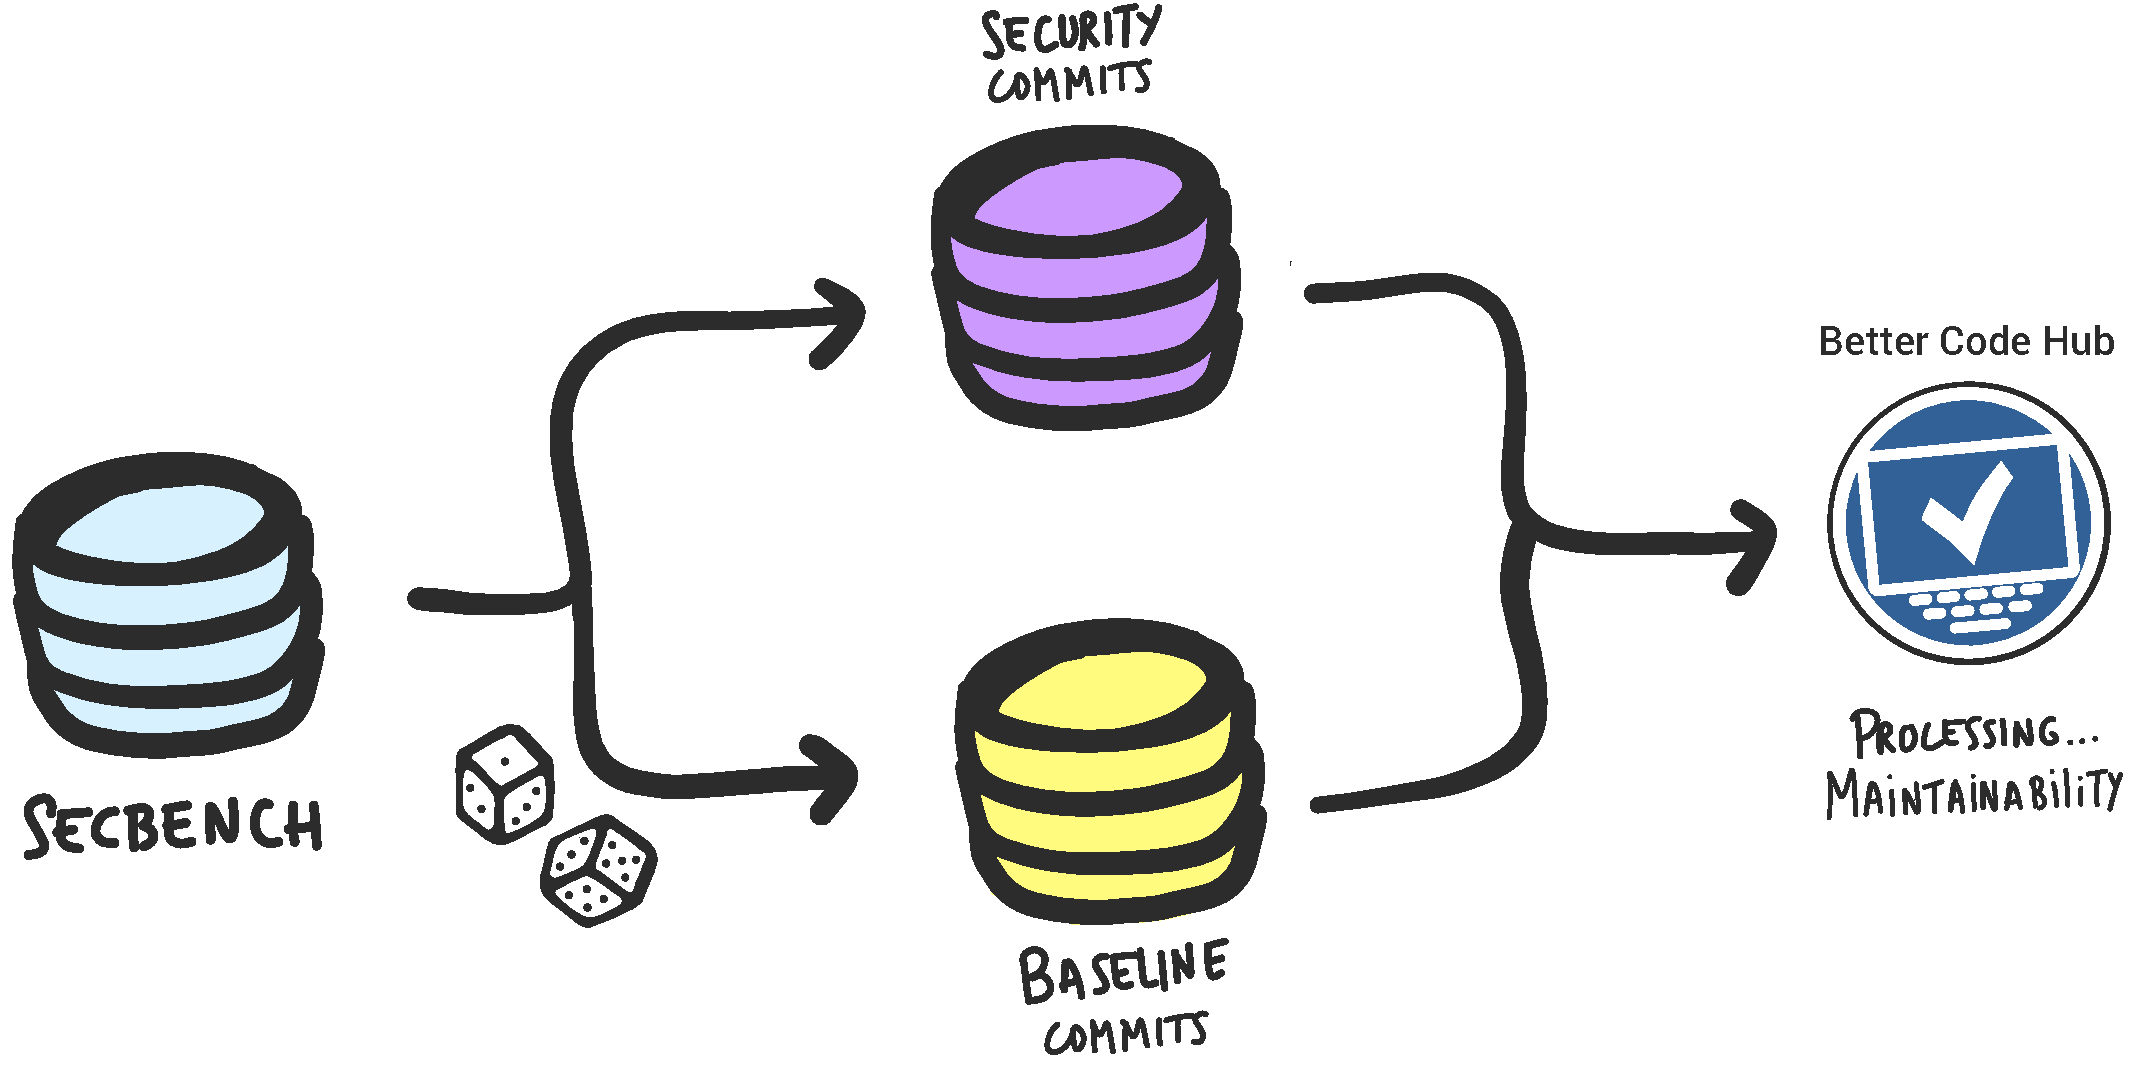
\includegraphics[width=0.5\textwidth]{figures/methodology.pdf}
 	\caption{Maintainability difference for security and baseline commits \textcolor{mypink3}{@update}}
	\label{fig:met}
\end{figure}

\subsection{Dataset}

To evaluate the impact of security refactorings on the maintainability of open-source software, we use a dataset of security flaws provided by a study conducted in 2017 \cite{Reis:2017:IJSSE} where the authors mined more than 248 GitHub repositories for several different patterns (e.g., injection, cross-site scripting, cross-site request forgery, memory leaks). Reis and Abreu (2017) mined open-source software aiming the extraction of real test cases - created by real developers on their daily basis development - to test and assess the performance of static analysis tools since using hand-seeded test cases or mutations could lead to misleading assessments of the tools' capabilities. The study yielded to a dataset of more than 600 test cases for 16 different patterns. Each test case of the dataset is a triplet of folders: the commit before the refactoring, the commit responsible for the refactoring and the snippets of code that differ from one version to another (usually, called \textit{diff}) - where one can easily identify the code used to fix the security flaw. In this study, we focus on computing the maintainability of the commits before and after the security refactoring to calculate if the impact was positive, negative or none.



\begin{table*}[h]
\centering
\caption{Descriptive statistics of the dataset projects\textcolor{mypink3}{@update}} \label{tab:dataset}
\begin{tabular}{@{}ccccccccccc@{}}
\toprule
     & forks   & stars   & watchers & contributors & commits  & branches & releases & size      & issues  & pull requests \\ \midrule
Mean & 1734.79 & 5262.97 & 395.11   & 152.48       & 22257.82 & 44.08    & 126.31   & 143243.64 & 3725.4  & 1976.92       \\
Min     & 1       & 3       & 1        & 0            & 103      & 1        & 0        & 108       & 0       & 0             \\
25 \%     & 374.75  & 1571.5  & 117.75   & 48           & 1347     & 4        & 22       & 8339.5    & 321.25  & 151.75        \\
Median     & 887     & 2836.5  & 258.5    & 102.5        & 5823     & 9        & 59       & 38331.5   & 1652.5  & 515.5         \\
75 \%     & 2196    & 6455.75 & 462.5    & 259          & 22786.25 & 22.25    & 142.25   & 164442.5  & 4152.75 & 1944.25       \\
Max     & 16366   & 31841   & 3446     & 413          & 717449   & 1227     & 1114     & 2042017   & 33970   & 19329         \\
Total     & 180418  & 547349  & 41091    & 15858        & 2314813  & 4584     & 13136    & 14897339  & 387442  & 205600        \\ \bottomrule
\end{tabular}
\end{table*}



\subsection{Security vs. Baseline Commits}



\subsection{Maintainability}






\section{Results}

\begin{figure}[h]
 	\centering
 	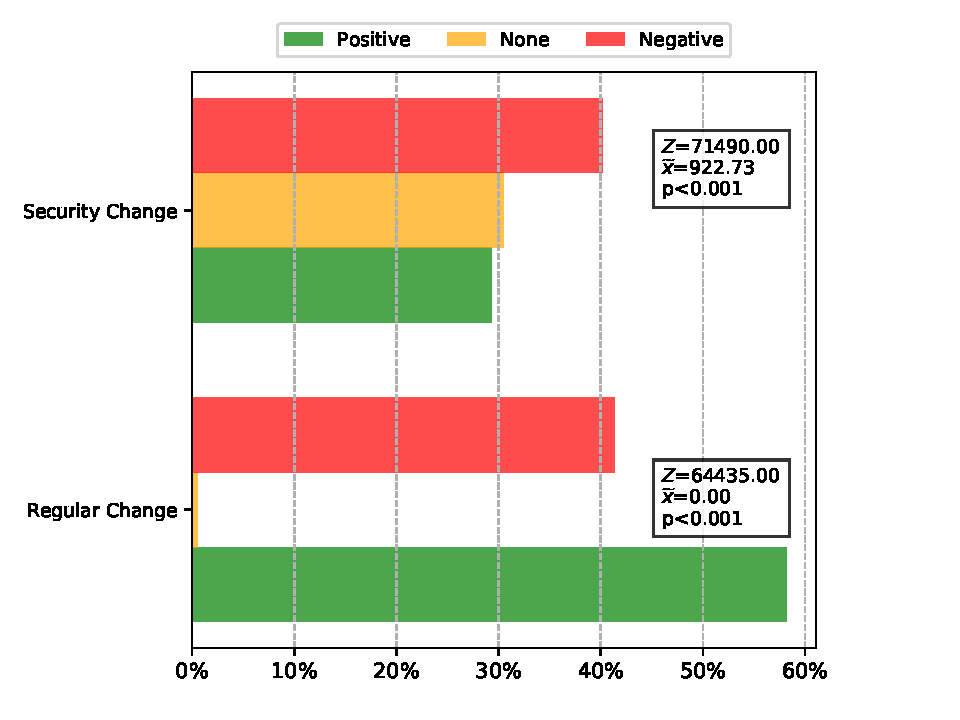
\includegraphics[width=0.4\textwidth]{figures/maintainability.pdf}
 	\caption{Maintainability difference for security and baseline commits \textcolor{mypink3}{@update}}
\end{figure}

\begin{figure}[h]
 	\centering
 	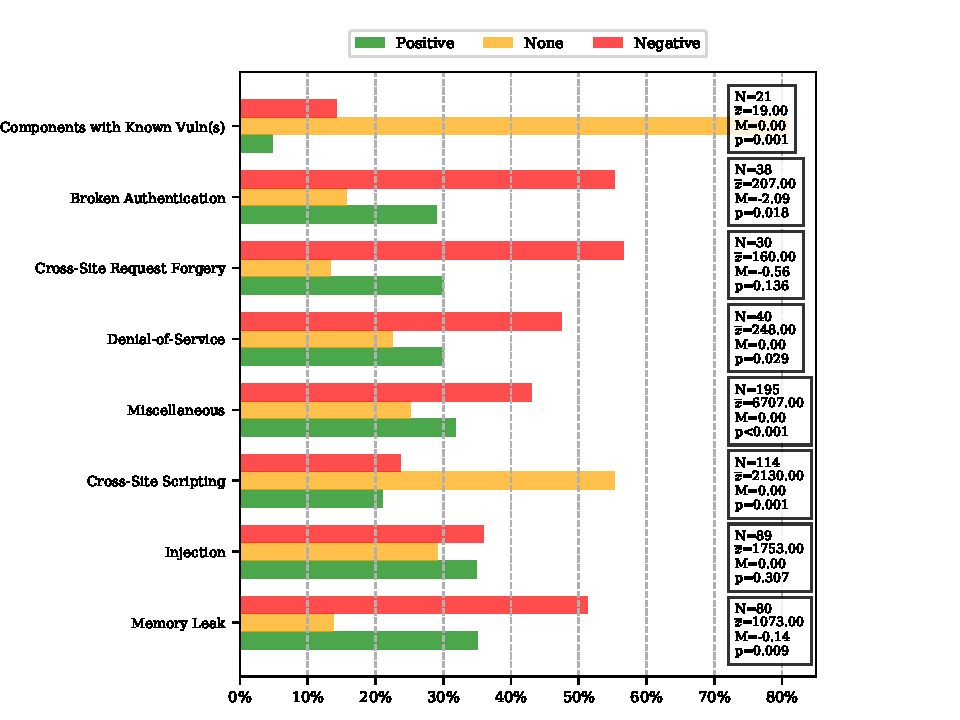
\includegraphics[width=0.55\textwidth]{figures/category.pdf}
 	\caption{Maintainability difference by type of security commit \textcolor{mypink3}{@update}}
\end{figure}



\begin{framed}
\textit{\textbf{RQ1} What is the impact of security refactorings on the maintainability of open-source software?}
\end{framed}

\begin{framed}
\textit{\textbf{RQ2} Which patterns of security refactorings are more likely to affect open-source software maintainability?}
\end{framed}

\section{Discussion}


\section{Threats to Validity}

\section{Related Work}


\section{Conclusion and Future Work}



\section*{Acknowledgment}

Better Code Hub?

{
 \bibliographystyle{IEEEtran}
  \bibliography{icpc19}
}

\end{document}
